\subsection{Round 1 Solutions}\label{S::2021-O-1}

\begin{resources}
    Review by \resit{https://www.youtube.com/watch?v=GhAYpBa6MkM}{Way Tan}
\end{resources}

\begin{question}[1741]\label{Q::2021-O-1-1}
    It is given that $\dfrac\pi2 < \b < \a < \dfrac{3\pi}{4}$, $\cos{\a - \b} = \dfrac{12}{13}$ and $\sin{\a + \b} = -\dfrac35$. Find $\floor{\abs{2021\sin{2\a}}}$.
\end{question}
\begin{solution*}
    Note that $\a - \b$ is in the first quadrant, while $\a + \b$ is in the third quadrant. Hence, $\sin{\a - \b} = \frac{5}{13}$, while $\cos{\a + \b} = -\frac45$. Thus, \[\sin{2\a} = \sin{\a + \b} \cos{\a - \b} + \cos{\a + \b} \sin{\a - \b} = -\frac{56}{65}.\] The required answer is hence 1741.
\end{solution*}

\begin{question}[99999]\label{Q::2021-O-1-2}
    Find the number of solutions of the equation $\abs{x - 3} + \abs{x - 5} = 2$.

    \noindent \textit{(Note: If you think that there are infinitely many solutions, enter your answer as ``99999''.)}
\end{question}
\begin{solution*}
    Observe that for all $x \in [3, 5]$, we have $\abs{x - 3} + \abs{x - 5} = 2$. There are hence infinitely many solutions.
\end{solution*}

\begin{question}[4290]\label{Q::2021-O-1-3}
    Evaluate $1 \times 2 \times 3 + 2 \times 3 \times 4 + 3 \times 4 \times 5 + \cdots + 10 \times 11 \times 12$.
\end{question}
\begin{solution*}
    We are tasked with evaluating $\displaystyle\sum_{k = 1}^{10} k(k+1)(k+2)$. Expanding, we have $\displaystyle\sum_{k = 1}^{10} k^3 + 3k^2 + 2k$. Using the standard formulae \[\sum_{k=1}^n k = \frac{k(k+1)}{2}, \qquad \sum_{k=1}^n k^2 = \frac{k(k+1)(2k+1)}{6}, \qquad \sum_{k=1}^n k^3 = \bp{\frac{k(k+1)}{2}}^2,\] we arrive at 4290.
\end{solution*}

\clearpage
\begin{question}[7]\label{Q::2021-O-1-4}
    It is given that the solution of the inequality $\sqrt{81 - x^4} \leq kx + 1$ is $a \leq x \leq b$ with $b - a = 2$, where $k > 0$. Determine $\floor k$.
\end{question}
\begin{solution*}
    Observe that $\sqrt{81 - x^4}$ is even, is defined only on $[-3, 3]$, and is decreasing for $x > 0$. It follows that $b = 3$, whence $a = 1$. However, at $x = a$, we have equality. Hence, $\sqrt{81 - 1^2} = k + 1$, immediately implying $\floor{k} = \floor{\sqrt{80} - 1} = 7$.
\end{solution*}

\begin{question}[1395]\label{Q::2021-O-1-5}
    The figure below shows a cross that is cut out from a $10 \times 9$ rectangular board.

    \begin{center}
        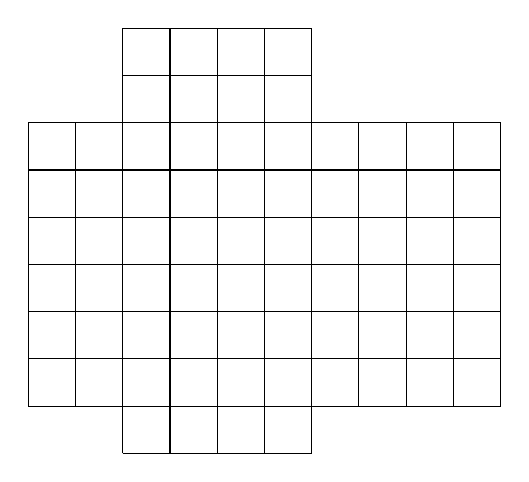
\begin{tikzpicture}[scale=0.6]
            \foreach \y in {1, 2, ..., 7}{
                \draw (0, \y) -- (10, \y);
            }

            \foreach \y in {0, 8, 9}{
                \draw (2, \y) -- (6, \y);
            }

            \foreach \x in {0, 1, 7, 8, 9, 10}{
                \draw (\x, 1) -- (\x, 7);
            }

            \foreach \x in {2, 3, ..., 6}{
                \draw (\x, 0) -- (\x, 9);
            }

        \end{tikzpicture}
    \end{center} Find the total number of rectangles in the above figure.

    \noindent\textit{(Note: A square is a rectangle.)}
\end{question}
\begin{solution*}
    Consider an $m \times n$ rectangular grid. Choosing a rectangle is equivalent to choosing 2 horizontal lines and two vertical lines (the four lines uniquely outline a rectangle). Since there are a total of $m+1$ horizontal lines and $n+1$ vertical lines, the number of rectangles in such a grid can be calculated as $\binom{m+1}{2} \binom{n+1}{2}$.

    Returning to our problem, the total number of rectangles in the figure is hence $\binom{11}{2} \binom{7}{2} + \binom{5}{2} \binom{10}{2} - \binom{5}{2} \binom{7}{2} = 1395$. Note that we subtracted $\binom{5}{2} \binom{7}{2}$ to account for the double-counting in the middle of the grid.
\end{solution*}

\begin{question}[2020]\label{Q::2021-O-1-6}
    Consider all polynomials $P(x, y)$ in two variables such that $P(0, 0) = 2020$ and for all $x$ and $y$, $P(x, y) = P(x + y, y - x)$. Find the largest possible value of $P(1, 1)$.
\end{question}
\begin{solution}
    Setting $x=0$ and relabelling $y$ as $x$, we get \[P(0, x) = P(x, x) \tag{1}.\] Setting $y = x$, we get \[P(x, x) = P(2x , 0).\] Setting $y = 0$, we get \[P(x, 0) = P(x, -x).\] Setting $y = -x$, we get \[P(x, -x) = P(0, -2x).\] We hence have \[P(0, x) = P(x, x) = P(2x, 0) = P(2x, -2x) = P(0, -4x),\] implying \[P(0, x) = P(0, -\tfrac14 x) \tag{2}.\] From (1), we have $P(1, 1) = P(0, 1)$. Using (2) repeatedly, we have \[P(0, 1) = P(0, -\tfrac14) = P(0, \tfrac1{16}) = \cdots = P(0, 0) = 2020.\] Thus, $P(1, 1) = 2020$.
\end{solution}
\begin{solution}[Abusing uniqueness]
    Suppose $k > 2020$ is the largest possible value of $P(1, 1)$. Then $k$ can be as big as we wish it to be. However, by the nature of the problem, $k$ should be unique. Hence, $k > 2020$ is impossible, implying that $2020$ is indeed the largest possible value of $P(1, 1)$ (occurring when $P(x, y) = 2020$ for all $x$, $y$).
\end{solution}

\begin{question}[16]\label{Q::2021-O-1-7}
    In the three-dimensional Cartesian space with $\vec i$, $\vec j$ and $\vec k$ denoting the unit vectors along three perpendicular directions in a clockwise manner, the line $l$ with equation given by $\vec r \crossp (\vec i + 2 \vec j + 3 \vec k) = 5\vec i - 13\vec j + 7\vec k$ intersects the plane $\Pi$ with equation $x + y + z = 16$ at the point $(a, b, c)$. Find the value of $a + b + c$.
\end{question}
\begin{solution*}
    $(a, b, c)$ lies on $\Pi$ and hence satisfies the equation $x + y + z = 16$. Hence, $a + b + c = 16$.
\end{solution*}

\begin{question}[169]\label{Q::2021-O-1-8}
    Find the minimum value of $(x + 7)^2 + (y + 2)^2$ subject to the constraint $(x-5)^2 + (y-7)^2 = 4$.
\end{question}
\begin{solution*}
    Let $(x + 7)^2 + (y + 2)^2 = r^2$, which describes a circle with centre $(-7, -2)$ and radius $r$. Meanwhile, $(x-5)^2 + (y-7)^2 = 4$ describes a circle with centre $(5, 7)$ and radius 2. The smallest $r$ occurs when the two circles are externally tangent. This implies that the sum of the radii is equal to the distance between their centres: $r + 2 = \sqrt{12^2 + 9^2}$. Hence, the minimum value is $r^2 = 169$.
\end{solution*}

\begin{question}[98]\label{Q::2021-O-1-9}
    Find the largest possible value $\a^4 + \b^4 + \g^4$ among all possible sets of numbers $(\a, \b, \g)$ that satisfy the equations
    \[\begin{aligned}
        \a + \b + \g &= 2\\
        \a^2 + \b^2 + \g^2 &= 14\\
        \a^3 + \b^3 + \g^3 &= 20.
    \end{aligned}\]
\end{question}
\begin{solution*}
    Newton's identities state that
    \begin{alignat*}{2}
        n \geq k \geq 1 :&& \qquad ke_k &= \sum_{i=1}^k (-1)^{i-1} e_{k-i} p_i\\
        k > n \geq 1 :&& 0 &= \sum_{i=k-n}^k (-1)^{i-1} e_{k-i} p_i
    \end{alignat*}
    where $e_k$ is the $k$th elementary symmetric polynomial of $n$ variables, and $p_k$ is the $k$th power sum of $n$ variables.
    
    In our case, we have $n=3$, along with \[e_0 = 1, \quad p_0 = 3, \quad p_1 = e_1 = 2, \quad p_2 = 14, \quad p_3 = 20,\] and we wish to find $p_4$. Evaluating the above sums at $k = 2, 3, 4$, we get
    \begin{alignat*}{2}
        k = 2 : && \quad2e_2 = e_1p_1 - e_0p_2 &\implies e_2 = -5\\
        k = 3 : && \quad 3e_3 = e_2p_1 - e_1p_2 + e_0p_3 &\implies e_3 = -6\\
        k = 4 : && \quad 0 = e_3p_1 - e_2p_2 + e_1p_3 - e_0p_4 &\implies p_4 = 98
    \end{alignat*}
    Hence, $\a^4 + \b^4 + \g^4 = 98$.
\end{solution*}

\begin{question}[6]\label{Q::2021-O-1-10}
    If $p$ is the product of all the non-zero real roots of the equation \[\sqrt[9]{x^7 + 30x^5} = \sqrt[7]{x^9 - 30x^5},\] find $\floor{\abs{p}}$.
\end{question}
\begin{solution*}
    Dividing through by $x$ and substituting $y = x^2$ yields \[\sqrt[9]{y^{-1} + 30y^{-2}} = \sqrt[7]{y - 30y^{-1}}.\] Observe that the LHS is decreasing while the RHS is increasing. There is hence at most one real root. Indeed, by inspection, $y = 6$ satisfies the equation. We hence have $x = \pm \sqrt 6$, whence $\floor{\abs{p}} = 6$.
\end{solution*}

\begin{question}[6]\label{Q::2021-O-1-11}
    Let $S$ be the sum of a convergent geometric series with first term 1. If the third term of the series is the arithmetic mean of the first two terms, find $\floor{3S + 4}$.
\end{question}
\begin{solution*}
    Let $r$ be the common ratio of the geometric series. Then we have $r^2 = (1+r)/2$, whence $r = -1/2$ (note that we reject $r = 1$ since the series is convergent). Hence, \[\floor{3S + 4} = \floor{3 \cdot \frac{1}{1 - (-1/2)} + 4} = 6.\]
\end{solution*}

\begin{question}[89]\label{Q::2021-O-1-12}
    Given that $\sin \a + \sin \b = \dfrac1{10}$, and $\cos \a + \cos \b = \dfrac19$, find $\floor{\tan[2]{\a + \b}}$.
\end{question}
\begin{solution*}
    By the sum-to-product identities, we have 
    \begin{align*}
        \sin \a + \sin \b &= 2\sin{\frac{\a+\b}{2}}\cos{\frac{\a - \b}{2}},\\
        \cos \a + \cos \b &= 2\cos{\frac{\a+\b}{2}}\cos{\frac{\a-\b}{2}}.
    \end{align*}
    Hence, $\tan{\frac{\a+\b}{2}} = \frac{1/10}{1/9} = \frac9{10}$. By the tangent double-angle identity, we finally get \[\floor{\tan[2]{\a + \b}} = \floor{\bp{\frac{2 \cdot 9/10}{1 - (9/10)^2}}^2} = 89.\]
\end{solution*}

\begin{question}[2]\label{Q::2021-O-1-13}
    Determine the number of positive integers that are divisible by 2021 and has exactly 2021 divisors (including 1 and itself).
\end{question}
\begin{solution*}
    Let $n = p_1^{d_1} \cdot p_2^{d_2} \cdots$, where $p_i$ are primes and $d_i$ are non-negative integers. The number of divisors of $n$ can be calculated as $(d_1 + 1)(d_2 + 1)\cdots$. Since 2021 only has two prime factors (43 and 47), there are only two possibilities, namely $(d_1, d_2) = (42, 46)$ or $(46, 42)$. Hence, $n$ has only two prime factors, which must be 43 and 47 (since $2021 \mid n$). Thus, there are two possibilities for $n$, namely $n = 43^{42} \cdot 47^{46}$ or $43^{46} \cdot 47^{42}$.
\end{solution*}

\begin{question}[2]\label{Q::2021-O-1-14}
    Let $S = \displaystyle\sum_{k=0}^{25} \binom{100}{4k} - 2^{98}$. Find $\floor{\abs{\dfrac{S}{2^{48}}}}$.
\end{question}
\begin{solution*}
    Let \[S_0 = \sum_{k=0}^{25} \binom{100}{4k}, \quad S_1 = \sum_{k=0}^{24} \binom{100}{4k+1}, \quad S_2 = \sum_{k=0}^{24} \binom{100}{4k+2}, \quad S_3 = \sum_{k=0}^{24} \binom{100}{4k+3}.\] Consider $(1 + x)^{100} = \displaystyle\sum_{k=0}^{100} \binom{100}{k} x^{k}$. Evaluating the binomial at $x = 1, i, -1, -i$, we have the following system of equations: \[\left\{
        \begin{aligned}
            (1+1)^{100} &= S_0 + S_1 + S_2 + S_3\\
            (1+i)^{100} &= S_0 + iS_1 - S_2 - iS_3\\
            (1-1)^{100} &= S_0 - S_1 + S_2 - S_3\\
            (1-i)^{100} &= S_0 - iS_1 - S_2 + iS_3
        \end{aligned}\right.\] Solving, one gets \[4S_0 = 2^{100} + (1+i)^{100} + (1-i)^{100} = 2^{100} + 2 \cdot 2^{100/2}\cos{100 \cdot \tfrac{\pi}4} = 2^{100} - 2^{51}.\] Hence, \[\floor{\abs{\frac{S}{2^{48}}}} = \floor{\abs{\frac{(2^{100} - 2^{51})/4 - 2^{98}}{2^{48}}}} = 2.\]
\end{solution*}

\begin{question}[1348]\label{Q::2021-O-1-15}
    Assume that $ABC$ is an acute triangle with $\sin{A + B} = \dfrac35$ and $\sin{A-B} = \dfrac15$. If $AB = 2022(\sqrt6 - 2)$, determine $\floor h$, where $h$ is the height of the triangle from $C$ on $AB$.
\end{question}
\begin{solution*}
    It is trivial to see that $AB = h(\cot A + \cot B)$. Since both $A$ and $B$ are acute, we have $\cos{A+B} = \frac45$ and $\cos{A-B} = \frac{2\sqrt{6}}{5}$. We thus have
    \begin{align*}
        2\cos A \cos B &= \cos{A + B} + \cos{A - B} = \frac{4 + 2\sqrt6}{5}\\
        2\sin A \cos B &= \sin{A + B} + \sin{A - B} = \frac45\\
        2\sin A \sin B &= \cos{A-B} - \cos{A+ B} = \frac{2\sqrt6 - 4}{5}
    \end{align*}
    It follows that $\cot A = \frac{2 + \sqrt6}{2}$ and $\cot B = \frac{2}{\sqrt6 - 2}$. Hence, \[2022(\sqrt 6 - 2) = h\bp{\frac{2 + \sqrt6}{2} + \frac{2}{\sqrt6 - 2}} \implies h = 1348.\]
\end{solution*}

\begin{question}[10]\label{Q::2021-O-1-16}
    Let $a_1, a_2, \cdots$ be a sequence with $a_1 = 1$ and $a_{n+1} = \dfrac{n+2}{n} S_n$ for all $n = 1, 2, \cdots$, where $S_n = a_1 + a_2 + \cdots + a_n$. Determine the minimum integer $n$ such that $a_n \geq 2021$.
\end{question}
\begin{solution*}
    We claim that $a_n = 2^{n-2} (n+1)$. We prove this via induction. Consider $a_2$ as the base case: from the given equation, $a_2 = \frac{1+2}{1}(a_1) = 3$, which clearly satisfies our claim. Suppose that $a_k = 2^{k-2} (k+1)$ for some positive integer $k$. We first show that $S_k = k2^{k-1}$. Observe that \[\sum_{i=1}^k x^i = \frac{x(1-x^k)}{1-x} \overset{\derx{}{x}}{\implies} \sum_{i = 1}^k ix^{i-1} = \frac{kx^{k+1} - (k+1)x^k + 1}{(1-x)^2}.\] Evaluating at $x = 2$, we have \[\sum_{i = 1}^k i2^{i-1} = k2^{k+1} - (k+1)2^k +1.\] Thus, \[S_k = \sum_{i=1}^k \bp{\frac12 \cdot i2^{i-1} + 2^{i-2}} = \frac12\bp{k2^{k+1} - (k+1)2^k +1} + \frac12 \bp{2^k - 1} = k2^{k-1}.\] This immediately implies \[a_{k+1} = \frac{k+2}{k} \cdot k2^{k-1} = (k+2)2^{k-1},\] closing the induction. It is hence easy to see that $\min n = 10$.
\end{solution*}

\begin{question}[101]\label{Q::2021-O-1-17}
    Each card of a stack of 101 cards has one side coloured red and the other coloured blue. Initially all cards have the red side facing up and stacked together in a deck. On each turn, Ah Meng takes 8 cards on the top, flip them over, and place them to the bottom deck. Determine the minimum number of turns required so that all the cards have the red sides facing up again.
\end{question}
\begin{solution*}
    Notice that the stack of cards can be represented by an array of numbers. Initially, all entries are 0. When a card is flipped over, the entry associated with that card is incremented by 1. The ``incrementer'' starts at the first entry and makes its way sequentially across the array, jumping back to the start once it reaches the end.

    The figure below shows the array after one turn: \[\underbrace{1,1,1,1,1,1,1,1}_{\text{the first 8 entries}},\underbrace{0,0,0,0,0,0,0,\ldots,0}_{\text{the remaining 93 entries}}\]
    
    Let $k$ be the sum of the entries. At any given turn, we clearly have $8 \mid k$ (since eight cards are flipped over in a single turn). Furthermore, by the construction of the ``incrementer'', there are at most two distinct numbers in the array, and their difference must be 1. However, when all the cards have the red sides facing up again, each entry must be even. Hence, all 101 entries have the same number, whence $101 \mid k$. The smallest $k$ is thus $8 \cdot 101 = 808$, which occurs after $808/8 = 101$ turns.
\end{solution*}

\begin{question}[88]\label{Q::2021-O-1-18}
    Let $ABC$ be a triangle with $AB = 10$ and $\dfrac{\cos A}{\cos B} = \dfrac{AC}{BC} = \dfrac43$. Let $P$ be a point on the inscribed circle of triangle $ABC$. Find the largest possible value of $PA^2 + PB^2 + PC^2$.
\end{question}
\begin{solution*}
    By inspection, it is obvious that $\triangle ABC$ is a $6-8-10$ right triangle, with $a = 6$, $b = 8$ and $c = 10$ (where $a$, $b$ and $c$ denote the sides opposite $A$, $B$ and $C$ respectively). From $[ABC] = rs$, we see that the inradius of $\triangle ABC$ is 2. Let $A(8, 0)$, $B(0, 6)$ and $C(0, 0)$. Then the incircle has equation \[(x-2)^2 + (y-2)^2 = 2^2. \tag{1}\] Our goal now is to maximize $PA^2 + PB^2 + PC^2$, which can be expressed as \[\bs{(x-8)^2 + y^2} + \bs{x^2 + (y-6)^2} + \bs{x^2 + y^2},\] where $(x, y)$ are subject to (1). We can rewrite the above expression as \[3\bs{(x-2)^2 + (y-2)^2} + 76 - 4x.\] Using (1), this simplifies to $88 - 4x$. The largest possible value of $PA^2 + PB^2 + PC^2$ is hence 88, where $P(0, 2)$.
\end{solution*}

\begin{question}[65]\label{Q::2021-O-1-19}
    A basket contains 19 apples labelled by the numbers $2, 3, \ldots, 20$, and 19 bananas labelled by the numbers $2, 3, \ldots, 20$. Ah Beng picks $m$ apples and $n$ bananas from the basket. However, he needs to ensure that for any apple labelled $a$ and any banana labelled $b$ that he picks, $a$ and $b$ are relatively prime. Determine the largest possible value of $mn$.
\end{question}
\begin{solution*}
    Let $[n]$ be the set of prime factors of $n$. For instance, $[18] = \bc{2, 3}$. The following table arranges all integers $n \in [2, 20]$ according to $[n]$:
    \begin{table}[h]
        \centering
        \begin{tabular}{|l|l|l|l|l|l|}
        \hline
        $[n]$ & $n$ & $[n]$ & $n$ & $[n]$ & $n$ \\ \hline
        (\textbf{2}) & 2, 4, 8, 16 & (\textbf{11}) & 11 & (\textbf{2,3}) & 6, 12, 18 \\ \hline
        (\textbf{3}) & 3, 9 & (\textbf{13}) & 13 & (\textbf{2,5}) & 10, 20 \\ \hline
        (\textbf{5}) & 5 & (\textbf{17}) & 17 & (\textbf{2,7}) & 14 \\ \hline
        (\textbf{7}) & 7 & (\textbf{19}) & 19 & (\textbf{3,5}) & 15 \\ \hline
        \end{tabular}
    \end{table}
    
    We now create two sets by combining the above sets. It seems clear that the largest set can be formed by grouping (2), (3), (5), $(2, 3)$, $(2, 5)$ and $(3, 5)$ together. This gives a set of size 13. By grouping the remaining sets (except for $(2, 7)$, since it would be in conflict with (2)), we get another set of size $5$. Hence, $\max mn = 13 \cdot 5 = 65$.
\end{solution*}

\begin{question}[25]\label{Q::2021-O-1-20}
    Let $p(x) = ax^2 - bx + c$ be a polynomial where $a$, $b$, $c$ are positive integers and $p(x)$ has two distinct roots in $(0, 1)$. Determine the least possible value of $abc$.
\end{question}
\begin{solution*}
    Since $p(x)$ has two distinct roots, its discriminant must be positive: \[b^2 - 4ac > 0. \tag{1}\] Furthermore, the two roots are in $(0, 1)$. By the quadratic formula, we have $\frac{b \pm \sqrt{b^2 - 4ac}}{2a} \in (0, 1)$, implying $\sqrt{b^2 - 4ac} \in [0, 2a-b)$. Squaring, we get $b^2 - 4ac < (2a-b)^2$, whence \[a > b - c.\tag{2}\] Since we wish to find the smallest value of $abc$, we fix $c = 1$. From (2), we see that $a = b$. (1) thus implies that $a = b = 5$, whence $abc = 25$.
\end{solution*}

\begin{question}[108]\label{Q::2021-O-1-21}
    In the triangle $ABC$, $\angle A > 90\deg$, the incircle touches the side $BC$ and $AC$ at $A_1$ and $B_1$ respectively. The line $A_1 B_1$ meets the extension of $BA$ at $X$ such that $CXB = 90\deg$. Suppose $BC^2 = AB^2 + BC \cdot AC$. Find the size of $\angle A$ in degrees.
\end{question}
\begin{center}
    \begin{tikzpicture}[scale=0.5, rotate=72]
        \coordinate[label=below:$A$] (A) at (-2.9, 0);
        \coordinate[label=below left:$B$] (B) at (-7.636, 14.477);
        \coordinate[label=above right:$C$] (C) at (12.332, 0);
        \coordinate[label=above left:$A_1$] (A1) at (2.348, 7.238);
        \coordinate[label=right:$B_1$] (B1) at (0, 0);
        \coordinate[label=below right:$X$] (X) at (-1.427, -4.50);
        \coordinate[label=below left:$O$] (O) at (0, 4);

        \draw (B) -- (X) -- (C) -- (B);
        \draw (A) -- (C);
        \draw (O) circle[radius=4];
        \draw (A) -- (A1);
        \draw (X) -- (A1);

        \fill (O) circle[radius=3pt];

        \tkzMarkSegment[pos=.5,mark=|](B,A1);
        \tkzMarkSegment[pos=.5,mark=|](A1,C);
        \tkzMarkSegment[pos=.5,mark=|](X,A1);
        \tkzMarkSegment[pos=.5,mark=|](B1,C);

        \draw pic [draw, angle radius=3mm, ""] {angle = B1--A--A1};
        \draw pic [draw, angle radius=4mm, ""] {angle = A1--A--B};

        \draw pic [draw, angle radius=3mm, ""] {right angle = A--A1--C};
        \draw pic [draw, angle radius=3mm, ""] {right angle = A--A1--B};
        \draw pic [draw, angle radius=3mm, ""] {right angle = A--X--C};

        \draw pic [draw, angle radius=5mm, ""] {angle = A--B--A1};
        \draw pic [draw, angle radius=6mm, ""] {angle = A--B--A1};

        \draw pic [draw, angle radius=5mm, ""] {angle = A1--X--A};
        \draw pic [draw, angle radius=6mm, ""] {angle = A1--X--A};

        \draw pic [draw, angle radius=5mm, ""] {angle = A1--C--A};
        \draw pic [draw, angle radius=6mm, ""] {angle = A1--C--A};

    \end{tikzpicture}
\end{center}
\begin{solution*}    
    Let $\t = \frac12 \angle A$, and let $O$ be the incentre of $\triangle ABC$. Since $OA$ bisects $\angle A$, we have $\angle BAO = \angle CAO = \t$. Since $BC$ and $AC$ are tangent to the circle, we get several equalities: $C A_1 = C B_1$, and $\angle BA_1 O = \angle CA_1O = 90\deg$. This immediately implies that $AOA_1$ is a straight line, thus $\triangle BA_1 A \equiv \triangle CA_1 A$, whence $BA_1 = CA_1 = C B_1$. Since $A_1$ is the midpoint of $BC$ and $\angle BXC = 90\deg$, it follows that $X A_1 = C A_1$. We thus have two isosceles triangles, namely $\triangle BA_1 X$ and $\triangle A_1 C B_1$.
    
    We now find two different expressions for $\angle A_1 B_1 C$. Firstly, we know that $\angle B_1 A X = 180\deg - 2\t$, while $\angle A_1XB = \angle A_1 B X = 90\deg - \t$ (using $\triangle B A_1 X$ isosceles), thus $\angle A_1 B_1 C = \angle AB_1 X = 3\t - 90\deg$.
    
    Secondly, we have $\angle ACB = \angle ABC = 90\deg - \t$ (using $\triangle BA_1 A \equiv \triangle CA_1 A$). Since $\triangle A_1 C B_1$ is isosceles, we have that $\angle A_1 B_1 C = 45\deg + \frac12 \t$.
    
    Thus, $3\t - 90\deg = 45\deg + \frac12 \t$, whence $\angle A = 2\t = 108\deg$.
\end{solution*}

\begin{question}[2021]\label{Q::2021-O-1-22}
    Find the number of positive integers $n$ such that $7n-16$ divides $n \cdot 13^{2019}$.
\end{question}
\begin{solution*}
    Observe that $7 \nmid 7n - 16$. Hence, $7n-16 \mid 7n \cdot 13^{2019} = (7n-16)\cdot13^{2019} + 16 \cdot 13^{2019}$. This gives $7n - 16 \mid 2^4 \cdot 13^{2019}$.

    \case{1} Suppose $7n-16 \leq 0$. Then $n = 1, 2$. Testing, we see that $n = 1$ fails ($-9 \nmid 13^{2019}$) while $n = 2$ works ($-2 \mid 2 \cdot 13^{2019}$).
    
    \case{2} Suppose $7n-16 > 0$. Then $7n-16$ is a factor of $2^4 \cdot 13^{2019}$. However, observe that $7n - 16 \equiv 5 \pmod 7$. It hence suffices to find the number of factors of $2^4 \cdot 13^{2019}$ that have a residue of 5 modulo 7.
    
    Let $7n-16 = 2^a \cdot 13^b$, where $a \leq 4$ and $b \leq 2019$ are non-negative integers. Note that $2^a \cdot 13^b \equiv 5 \pmod{7}$ if and only if $a = 1, 4$ and $b$ is odd. This gives $2 \cdot 2020/2 = 2020$ solutions in this case.
    
    Thus, there are a total of $2020 + 1 = 2021$ positive integers $n$ that satisfy the given condition.
\end{solution*}

\begin{question}[75]\label{Q::2021-O-1-23}
    In the acute triangle $ABC$, $P$ is a point on $AB$, $Q$ is a point on $AC$ such that $BP + CQ = PQ$. The bisector of $\angle A$ meets the circumcircle of the triangle $ABC$ at the point $R$ distinct from $A$. Suppose $\angle PRQ = 52.5\deg$. Find the size of $\angle BAC$ in degrees.
\end{question}
\begin{center}
    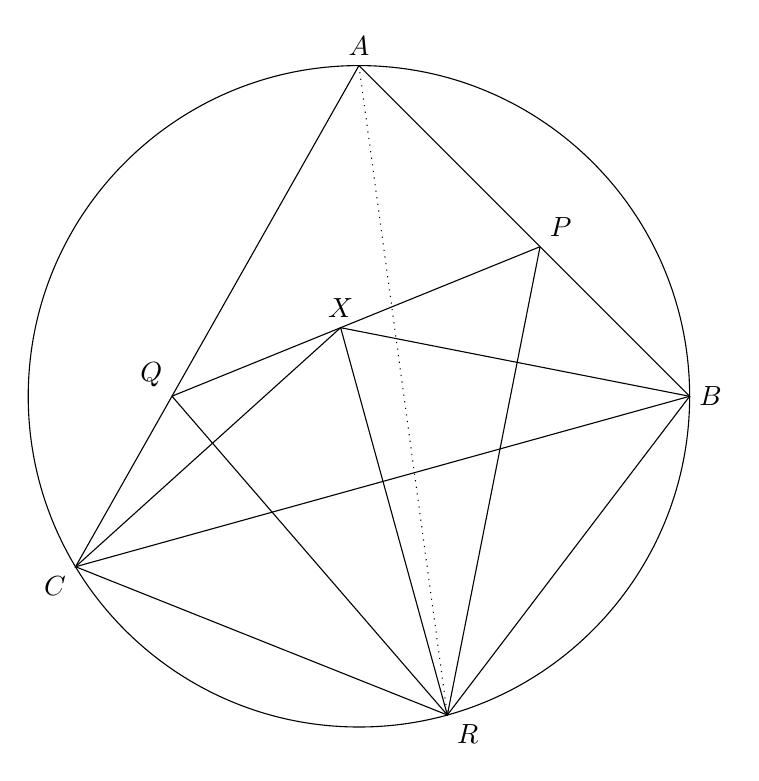
\begin{tikzpicture}[scale=0.7]
        \coordinate[label=above:$A$] (A) at (0, 6);
        \coordinate[label=right:$B$] (B) at (6, 0);
        \coordinate[label=below left:$C$] (C) at (-5.141, -3.092);
        \coordinate[label=above right:$P$] (P) at (3.286, 2.714);
        \coordinate[label=above left:$Q$] (Q) at (-3.392, 0.002);
        \coordinate[label=above:$X$] (X) at (-0.332, 1.245);
        \coordinate[label=below right:$R$] (R) at (1.604, -5.782);

        \draw (A) -- (B) -- (C) -- (A);
        \draw (P) -- (Q);
        \draw (C) -- (X);
        \draw (B) -- (X);
        \draw (X) -- (R);
        \draw[dotted] (A) -- (R);
        \draw (C) -- (R) -- (B);
        \draw (P) -- (R) -- (Q);

        \draw (0, 0) circle[radius=6];

        \tkzMarkSegment[pos=.5,mark=|](C,Q);
        \tkzMarkSegment[pos=.5,mark=|](Q,X);
        \tkzMarkSegment[pos=.5,mark=||](X,P);
        \tkzMarkSegment[pos=.5,mark=||](P,B);
        \tkzMarkSegment[pos=.5,mark=|||](C,R);
        \tkzMarkSegment[pos=.5,mark=|||](R,X);
        \tkzMarkSegment[pos=.5,mark=|||](R,B);
    \end{tikzpicture}
\end{center}
\begin{solution*}
    By the incenter-excenter lemma, we have $CR = RB$. Let $X$ be the point on $PQ$ such that $CQ = QX$ and $XP = PB$. Note that $\angle XQC + \angle XPB = 180\deg + \angle A$. Since $\triangle CXQ$ and $\triangle XBP$ are both isosceles, it follows that $\angle QXC + \angle PXB = 90\deg - \frac12 \angle A$. Hence, $\angle CXB = 90\deg + \frac12 \angle A$. Also, since $ABRC$ is cyclic, $\angle CRB = 180\deg - \angle A$, whence reflex $\angle CRB = 180 \deg + \angle A = 2\angle CXB$. Hence, $R$ is the circumcentre of $\triangle CXB$, implying that $RX = CR = RB$. Thus, $QCXR$ and $PXBR$ are kites, hence $\angle QRX = \angle QRC$, and $\angle PRX = \angle PRB$. Thus, $\angle CRB = 2\angle PRQ = 105\deg$, whence $\angle A = 180\deg - 105\deg = 75\deg$.
\end{solution*}

\begin{question}[6]\label{Q::2021-O-1-24}
    Let $S = \displaystyle\int_{-\infty}^\infty e^{-\frac12 x^2} \d x$. Determine the value of $\floor{S^2}$.
\end{question}
\begin{solution*}
    The generalized Gaussian integral $\int_{-\infty}^\infty e^{-k x^2} \d x$ evaluates to $\sqrt{\pi/k}$. Hence, $\floor{S^2} = \floor{2\pi} = 6$.
\end{solution*}

\begin{question}[5]\label{Q::2021-O-1-25}
    Let $p$, $q$, $r$ be positive numbers with $p-r= 4q$ and $a_1, a_2, \cdots$ and $b_1, b_2, \cdots$ be two sequences defined by $a_1 = p$, $b_1 = q$ and for $n \geq 2$, \[a_n = pa_{n-1}, \quad b_n = qa_{n-1} + rb_{n-1}.\] Find the value of $\displaystyle\lim_{n \to \infty} \dfrac{\sqrt{a_n^2 + (3b_n)^2}}{b_n}$.
\end{question}
\begin{solution*}
    Observe that $a_n$ is simply a geometric series, with $a_n = p^n$. Hence, $b_n = qp^{n-1} + rb_{n-1}$. We now claim that $b_n = \frac14 \bp{p^n - r^n}$. We prove this via induction. Observe that the base case $b_1 = q = \frac14 (4q) = \frac14 \bp{p^1 - r^1}$ holds. Suppose that $b_k = \frac14 \bp{p^k - r^k}$ for some positive integer $k$. Then
    \begin{align*}
        b_{k+1} &= qp^{k} + r\bs{\frac14 \bp{p^k - r^k}} = \frac14 \bp{p-r} p^{k} + \frac14 r p^k - \frac14 r^{k+1}\\&= \frac14 \bp{p^{k+1} - rp^{k} + rp^k - r^{k+1}} = \frac14 \bp{p^{k+1} - r^{k+1}},
    \end{align*}
    closing the induction. The limit hence evaluates to
    \begin{align*}
        &\lim_{n \to \infty} \dfrac{\sqrt{a_n^2 + (3b_n)^2}}{b_n} = \lim_{n \to \infty} \sqrt{\bp{\frac{a_n}{b_n}}^2 + 9} = \lim_{n \to \infty} \sqrt{\bp{\frac{p^n}{\bp{p^n - r^n}/4}}^2 + 9} = \sqrt{4^2 + 9} = 5.
    \end{align*}
\end{solution*}